\documentclass{article}
\usepackage{graphicx}
\usepackage{amsmath}
\usepackage{amssymb}
\usepackage[italicdiff]{physics}
\usepackage{enumerate}
\usepackage{microtype}
\DisableLigatures{encoding= *, family=*}
\usepackage{titlesec}
\usepackage{xfrac}
\setcounter{secnumdepth}{4}
\usepackage{xcolor}
\usepackage[bookmarks=false]{hyperref}
\usepackage{mathtools}
\usepackage{tikz} 
\newcommand*\fullcirc[1][0.3ex]{\tikz\fill (0,0) circle (#1);} 
\usepackage{bigints}
\hypersetup{
    colorlinks=true,
    linkcolor=[RGB]{59 108 209},
    urlcolor=[RGB]{59 108 209}
}
\urlstyle{same}

\titleformat{\paragraph}
{\normalfont\normalsize\bfseries}{\theparagraph}{1em}{}
\titlespacing*{\paragraph}
{0pt}{3.25ex plus 1ex minus .2ex}{1.5ex plus .2ex}

\title{Formation of Girgnard's Reagent}
\author{}
\date{}

\begin{document}
\maketitle

\section{Reaction and Mechanism}
\begin{center}
    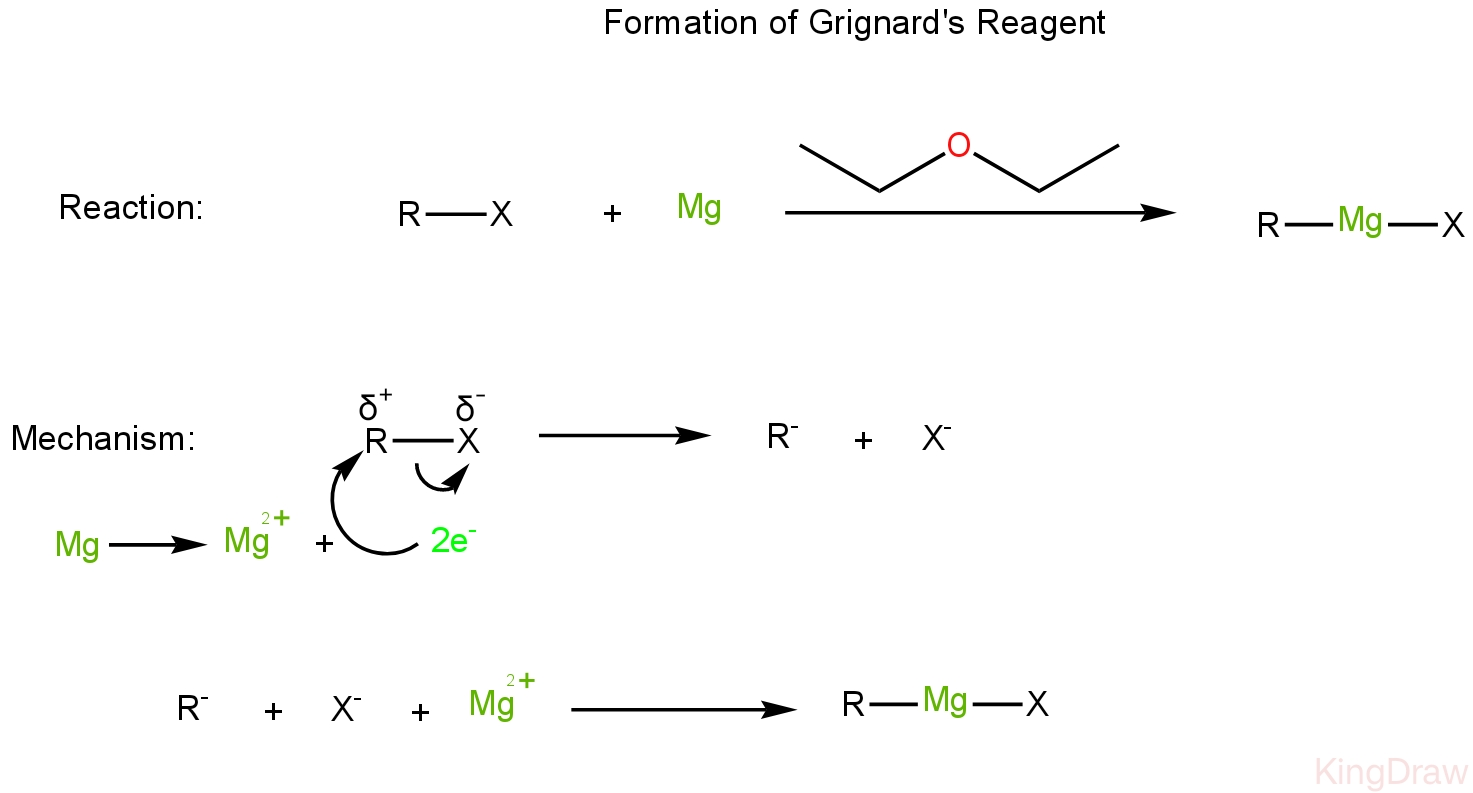
\includegraphics[scale=0.25]{FormationofGrignard'sReagent_1722171477216.JPEG}
\end{center}
\section{Reaction Observations}
\begin{enumerate}[i.]
    \item $C^-$ and $C^{\fullcirc}$ obtained as intermediate.
    \item $RMgX$ is also known as Organometallic Compound due to $\prescript{12}{6}{C}$ metal bond.
    \item $ROR$ for $RX$, $RI>RBr>RCl$
    \item Reaction doesn't occur in $RF$
    \item Dry $Et_{2}O$ or $THF$ is used as solvent.
\end{enumerate}
\end{document}